% ================================================================
%  DSC 208R -- Data Management for Analytics
%  Cloud Computing (Part 2): Comprehensive Review
%  Source: "Data Engineering for ML -- Cloud Computing Part 2"
% ================================================================
\documentclass[11pt]{article}

% -------------------- Packages --------------------
\usepackage[utf8]{inputenc}
\usepackage{amsmath,amssymb,amsfonts}
\usepackage{graphicx}
\usepackage{booktabs}
\usepackage{tikz}
\usetikzlibrary{positioning}
\usepackage{enumitem}
\usepackage{hyperref}
\usepackage{caption}
% -------------------- Packages --------------------
\usepackage[utf8]{inputenc}
\usepackage{amsmath,amssymb,amsfonts}
\usepackage{graphicx}
\usepackage{booktabs}
\usepackage{tikz}
\usetikzlibrary{positioning}
\usepackage{enumitem}
\usepackage{hyperref}
\usepackage{caption}
% -------------------- Packages --------------------
\usepackage[utf8]{inputenc}
\usepackage{amsmath,amssymb,amsfonts}
\usepackage{graphicx}
\usepackage{booktabs}
\usepackage{tikz}
\usetikzlibrary{positioning}
\usepackage{pgfplots}
\usepackage{enumitem}
\usepackage{listings}
\usepackage{hyperref}
\usepackage{caption}
\pgfplotsset{compat=1.17}

% -------------------- Document --------------------
\begin{document}

\begin{center}
  {\LARGE\bfseries Cloud Computing -- Part 2}\\[1.5mm]
  {\large Comprehensive Review}\\[0.7mm]
  {\normalsize DSC 208R -- Parallel Data Processing and the Cloud}
\end{center}
\vspace{-0.6em}\hrule\vspace{0.9em}

\tableofcontents
\newpage

% ================================================================
\section{Motivation}

Fixed bundles of CPU, memory, and storage can leave some resources under-used.  
Cloud providers therefore offer finer-grain renting models, notably
serverless Function as a Service (FaaS), to boost resource efficiency and cut cost by up to 10x compared to spot instances.:contentReference[oaicite:0]{index=0}

% ================================================================
\section{Serverless Paradigm}

\begin{itemize}[itemsep=0pt]
  \item User supplies a function and a resource hint (CPU, RAM).
  \item Provider handles provisioning, autoscaling, and teardown.
  \item Billing is by the millisecond of execution and GB-s of memory.
\end{itemize}

\subsection*{Car Analogy}

Owning a car is like on-prem hardware.  
Ride-sharing on demand is like serverless: you pay only for miles driven.:contentReference[oaicite:1]{index=1}

% ================================================================
\section{Example AWS Workloads}

\begin{enumerate}[itemsep=0pt]
  \item Athena -- serverless SQL over S3, schema on read, pay per TB scanned.
  \item Predictive data science -- SageMaker plus Data Lake for serverless ML training and inference.
  \item IoT pipeline -- edge devices stream data to SageMaker Neo models for real-time inference.:contentReference[oaicite:2]{index=2}
\end{enumerate}

% ================================================================
\section{Resource Disaggregation}

Logical next step: detach compute, memory, and storage so each is network attached and elastically added or removed in real time.

\begin{figure}[h]
  \centering
  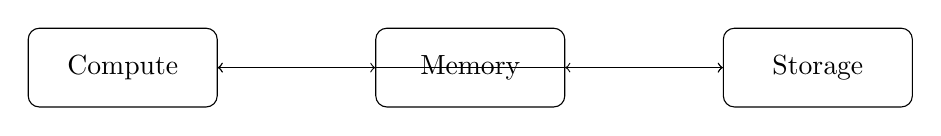
\begin{tikzpicture}[
    node/.style={draw,rounded corners,minimum width=2.4cm,minimum height=1cm},
    yshift=-0.2cm
  ]
    \node[node] (cpu) {Compute};
    \node[node,right=2.0cm of cpu] (mem) {Memory};
    \node[node,right=2.0cm of mem] (stor) {Storage};

    \draw[<->] (cpu) -- (mem);
    \draw[<->] (mem) -- (stor);
    \draw[<->] (cpu) -- (stor);
  \end{tikzpicture}
  \caption{All resources network attached and elastic.}
\end{figure}

Ongoing research aims to hot-plug new CPUs or RAM with sub-second latency.:contentReference[oaicite:3]{index=3}

% ================================================================
\section{Is All This Complexity Worth It?}

\begin{itemize}[itemsep=0pt]
  \item Pros of cloud: manageability, elastic capacity, pay-as-you-go cost.
  \item Cons of cloud: API complexity, long-term spend crossover, accidental waste, vendor lock-in, privacy and downtime risks.:contentReference[oaicite:4]{index=4}
\end{itemize}

Large enterprises, health care, and academia still rely on on-prem clusters or hybrid clouds to balance these trade-offs.

% ================================================================
\section{State of the Cloud Surveys}

Flexera surveys show

\begin{itemize}[itemsep=0pt]
  \item Public cloud adoption continues to rise each year.
  \item Multi-cloud strategies are common.
  \item Top challenge is controlling cost and cloud spend.:contentReference[oaicite:5]{index=5}
\end{itemize}

\begin{figure}[h]
  \centering
  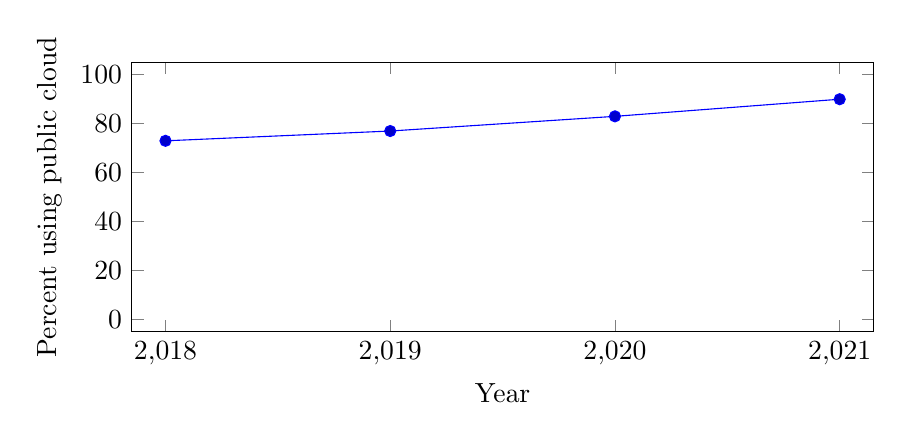
\begin{tikzpicture}
    \begin{axis}[
      width=11cm,
      height=5cm,
      xlabel=Year,
      ylabel=Percent using public cloud,
      ymin=0,ymax=100,
      xtick=data,
      ytick={0,20,40,60,80,100},
      enlargelimits=0.05
    ]
      \addplot+[mark=*] coordinates {(2018,73) (2019,77) (2020,83) (2021,90)};
    \end{axis}
  \end{tikzpicture}
  \caption{Trend in public cloud adoption (illustrative numbers).}
\end{figure}

% ================================================================
\section{Pros and Cons Summary}

\begin{itemize}[itemsep=0pt]
  \item \textbf{Pros}
    \begin{itemize}[itemsep=0pt]
      \item No hardware maintenance.
      \item Fine-grained cost aligned with use.
      \item Rapid scale up and down.
    \end{itemize}
  \item \textbf{Cons}
    \begin{itemize}[itemsep=0pt]
      \item Complex APIs and licenses; need CloudOps expertise.
      \item Long-term cost can exceed on-prem clusters.
      \item Vendor lock-in, outages, privacy and governance risks.
    \end{itemize}
\end{itemize}

% ================================================================
\section{Future Directions}

\begin{itemize}[itemsep=0pt]
  \item Fully disaggregated clouds with sub-second elasticity.
  \item Automatic budget guards and cost observability tools.
  \item Cross-vendor orchestration to reduce lock-in risk.
\end{itemize}

% ================================================================
\section*{Conclusion}

Cloud Computing Part 2 underscores how serverless and resource disaggregation push the pay-as-you-go vision, yet introduce new complexity and risk.  
Choosing between on-prem, hybrid, and cloud-native architectures requires careful cost, performance, and governance analysis.:contentReference[oaicite:6]{index=6}

\end{document}
